\section{Episode 69: Welcome to the Shit Show (NOICE)}

\medskip

\DndDropCapLine{I}n the chaotic emotion fuelled moments following Riphards execution of Kolo Exme seems to try to slink off with Kolo’s corpse. After all this darkness everyone’s thought is simply on seeing daylight again. Bernie tries to follow her, but she calmly asks him to remain with the rest of the group which sorely needs his wisdom, knowledge, and goodness. He debates his virtues to himself, but ultimately takes Exme’s kind and generous words to heart.\medskip

Burnie hides a package Exme seemingly gave him before anyone else can notice. Myron sternly expresses consternation that Exme thinks she can just walk away after the bullshit she just pulled, but Burnie talks him out of following her… for now.\medskip

Debate turns to tactics now that we find ourselves in a hostile city, wanted by the church authorities and entirely broken as a group and as people.\medskip

A deathly silence befalls the group as we trudge back through the sewers, searching for what little light remains in the world. Riphard carries his two weans, seemingly trying to shut out any thoughts about the situation at last and what remains of Delilah. Occasionally a smile does seem to flash across his face, buried deep behind the anger and shock. Myron carries Delilah’s corpse, her feet dragging along the floor as even her headless corpse dwarfs Myron’s diminutive stature.\medskip

Myron writes Rolltop Candian a letter warning him with evidence about the Inquisitors and begging him to reconsider his position and attitude in this new light.\medskip

Burnie sources a cart and tarpaulin, ever resourceful, and stashes the dead, hidden in plain sight. We slip out of the city boundaries under the cover of darkness, all there ever seems to be these days.\medskip

We reach Burnie’s parents house, who implore us inside. Myron resists and Burnie’s skepticism is raised at the sound of an apparently enthusiastic Mother he has never known. It seems she is just excited to share some news, someone is here to see him. His son!\medskip

“5ft 4? Covered in feathers?”\medskip

“That’s the one!”\medskip

“Never met him”\medskip

Burnie jokes and confesses this is indeed his son. He heads inside. Riphard wonders if he has news of the Tiger’s death. Riphard and Myron head onto the airship: Riphard silently taking his babies into his rooom with a loud clunk as he locks the door. Myron drowns his sorrows at the bar. He feels a comforting embrace on his shoulder: Captain Stick has fallen over onto him. Myron eyes the apparently inanimate stick with suspicion.\medskip

Burnie walks into his childhood home and the sight of his birdson drinking tea with his father greets his eyes warmly after the days horror. He has a request for Burnie. Burnie doesn’t know if he’s in a position to help what with the prostate related news he received last time he was home several years ago. Bucky says Burnie doesn’t know much about him, blunt but fair.\medskip

He explains that he trains the young assassins at the assassins guild. He says he has a final year student doing his final year thesis and exam to become a full blown assassin and thinks he needs experience in the wider world, and was wondering if they could join the group for a while. Burnie explains the whole murder church thing, but this doesn’t perturb Bucky from the idea. He explains he’s a VERY promising student and presses the matter.\medskip

Out from the shadows appears Christopher Mintz-Plasse the young assassin: Kevin. He tries to introduce himself to Burnie, but Burnie shuts him down spouting various contradictory and aggressive rules and suggestions. The young assassin tries to scribble these down and obey more than he disobeys, Burnie tells him not in infringe his personal right to privacy. He half burns his notebook.\medskip

Bucky asks why Burnie is covered in shit. He says he watched his best friend die at the hands of his least favourite acquaintance. Riphard sheds a tear in his room.\medskip

Burnie tells his parents to join the group as we have need for babysitters. The Dad is resistant to leave having just moved a few months ago, from the house next door. His mother requires little convincing though, especially at the mention of wee half-dwarf babies in need. Burnie tells Kevin to head to the basement and grab the biggest barrels of sherry he can.\medskip

Myron lobs a bottle at Kevin’s head as he boards the ship.\medskip

“FUCK OFF!”.\medskip

“Fucking hell!” ejaculates Kevin.\medskip

Burnie scolds Kevin for swearing. Kevin asks if we’re pirates, but Burnie tells him not everything is as it seems at first glance. Kevin tries to write this down in his half burnt notebook.\medskip

Burnie walks onto the ship and is greeted with several more bottles. Myron just froths at the mouth spitting out the odd “Fucking….” through his grenadine fueled rage.\medskip

“This ain’t one in one out mate”.\medskip

“Uh… I’m Kevin.”\medskip

Burnie tries to convince Myron to accept the youngling. Myron presses Burnie on where he stands. Burnie effuses about the situation, and accepts the reasons for Kolo’s death, but thinks the way it ultimately went down was murder. Kevin tries to chip in but Burnie shouts him down. “Against the church and on the side of the Gods” is his ultimate answer. Myron stammers out a rare confession that Burnie is right. The tension eases and Myron heads to bed.\medskip

Riphard is distractedly playing with the kids in his room, dangling toys at them and engaging where he can between vivid flashes of memory from the entire cursed time since he should’ve died. He has little sense of the time passing.\medskip

Burnie introduces Kevin to Captain Stick. Kevin salutes the stick. Burnie directs his parents to the empty master suite. Burnie insists everyone go the fuck to sleep. Kevin is resistant “But it’s 4pm sir” “DO I LOOK LIKE I KNOW WHAT A POST MERIDIAN IS?!” Burnie watches until Kevin goes to sleep, then gets the Cube Puzzle Die of Rubrex, which was in the package given to him by Exme along with a letter. He inspects it carefully with his built in hook lighter. He doesn’t set it on fire, which is a good start. He makes out a couple of words, but will have to wait before fully deciphering it. He nods off.\medskip

The group awaken in the familiar waiting room of Lazarus. Riphard has his kids in his arms. Kevin is exasperated he’s now apparently dreaming about Burnie. “This ain’t a dream lad”. Meredith elephants into the room and gives the group fizzy cold Bovril to drink. Kevin tries to wake himself up unsuccessfully.\medskip

The group are ushered in to see Laz. Meredith picks up Kevin and takes him through. Kevin talks to himself to remain calm.\medskip

Laz greets the group and expresses surprise at the lack of Exme and Kolo and the new faces. Myron asks Laz if he’s seen any of the various dead Goblin or Delilah come through. He tells Meredith to see who’s in the waiting lounge. Myron drunkenly exclaims despair at how it’s all gone to shit.\medskip

Burnie bluntly explains the situation to Laz. Myron shunders fizzy lurid pink Bovril vomit. He explains Kevin too. A lot has changed in a short space of time. Laz welcomes Kevin to hell and to the team. The group all ask for various cups of things at the revelation Laz can bring us cups of whatever we want. Kevin looks out of the window, but is wise beyond his years and retains his sanity, waving hello to the various murderers, thieves, and scallywags he recognises having assassinated recently.\medskip

There’s a big conversation here about how shitty Kolo was and how he’s now somewhere worse than hell because of the Kalimar stuff. Riphard is happy at this, Laz seems less pleased. Myron seems conflicted.\medskip

A fax comes in. Delilah is downstairs and will be held in the waiting room downstairs. There is no word of Kolo or the other Kalimar infected Goblin souls. Riphard is happy at the news and playfully bounces Dildo and Bildo on his knees.\medskip

Kevin tries to fly out of the window, thinking he’s still in his own dream and has any control over the situation. He screams for eternity before falling back in through the window from above. This should provide some good source material for his dissertation.\medskip

Laz tells us that speed is of the essence now that all the church wheels are in motion. We must travel to Lindedorf to find someone who can make us weapons to fight the church on our own. He explains that Kiros is not yet dead and may yet be saved. It’s time to bring the fight to the church. Post haste.\medskip

Laz tells me I need to nurture my children and they will grow up into great people as they have been touched by the Gods. It’s a little on the creepy side.\medskip

Laz tells Kevin if he doesn’t help us he will damn his soul to hell for an infinite amount of time longer than the infinite fall out of the window he just experienced. He clicks everyone back awake.\medskip

The group awake to Myron attempting to steer the ship, having tied up Captain Stick. Burnie wrestles the ship back under control. Myron goes to see Riphard and somberly asks what we are going to do about Burnie. The two agree he has to die, the question is when. An initial attempt at a signal is attempted, but needs further work.\medskip

Myron hates sherry. Burnie leaves Myron the note left from Exme that simply says: “I thought I could have both of you.”\medskip

Burnie plays with the puzzle die and thinks he’s getting somewhere, but accidentally triggers “Apprentice Security Mode”, locking down completely and is unusable for 24 hours. An idiot-proof mode fit for the user.\medskip

Kevin introduces himself to Riphard. Riphard is blunt and not exactly talkative. “Welcome to the shit show” summing up his general feelings and he walks off.\medskip

The airship trundles on to Lindedorf, just as Lazarus directed.\medskip

\vspace*{5mm}

\begin{center}
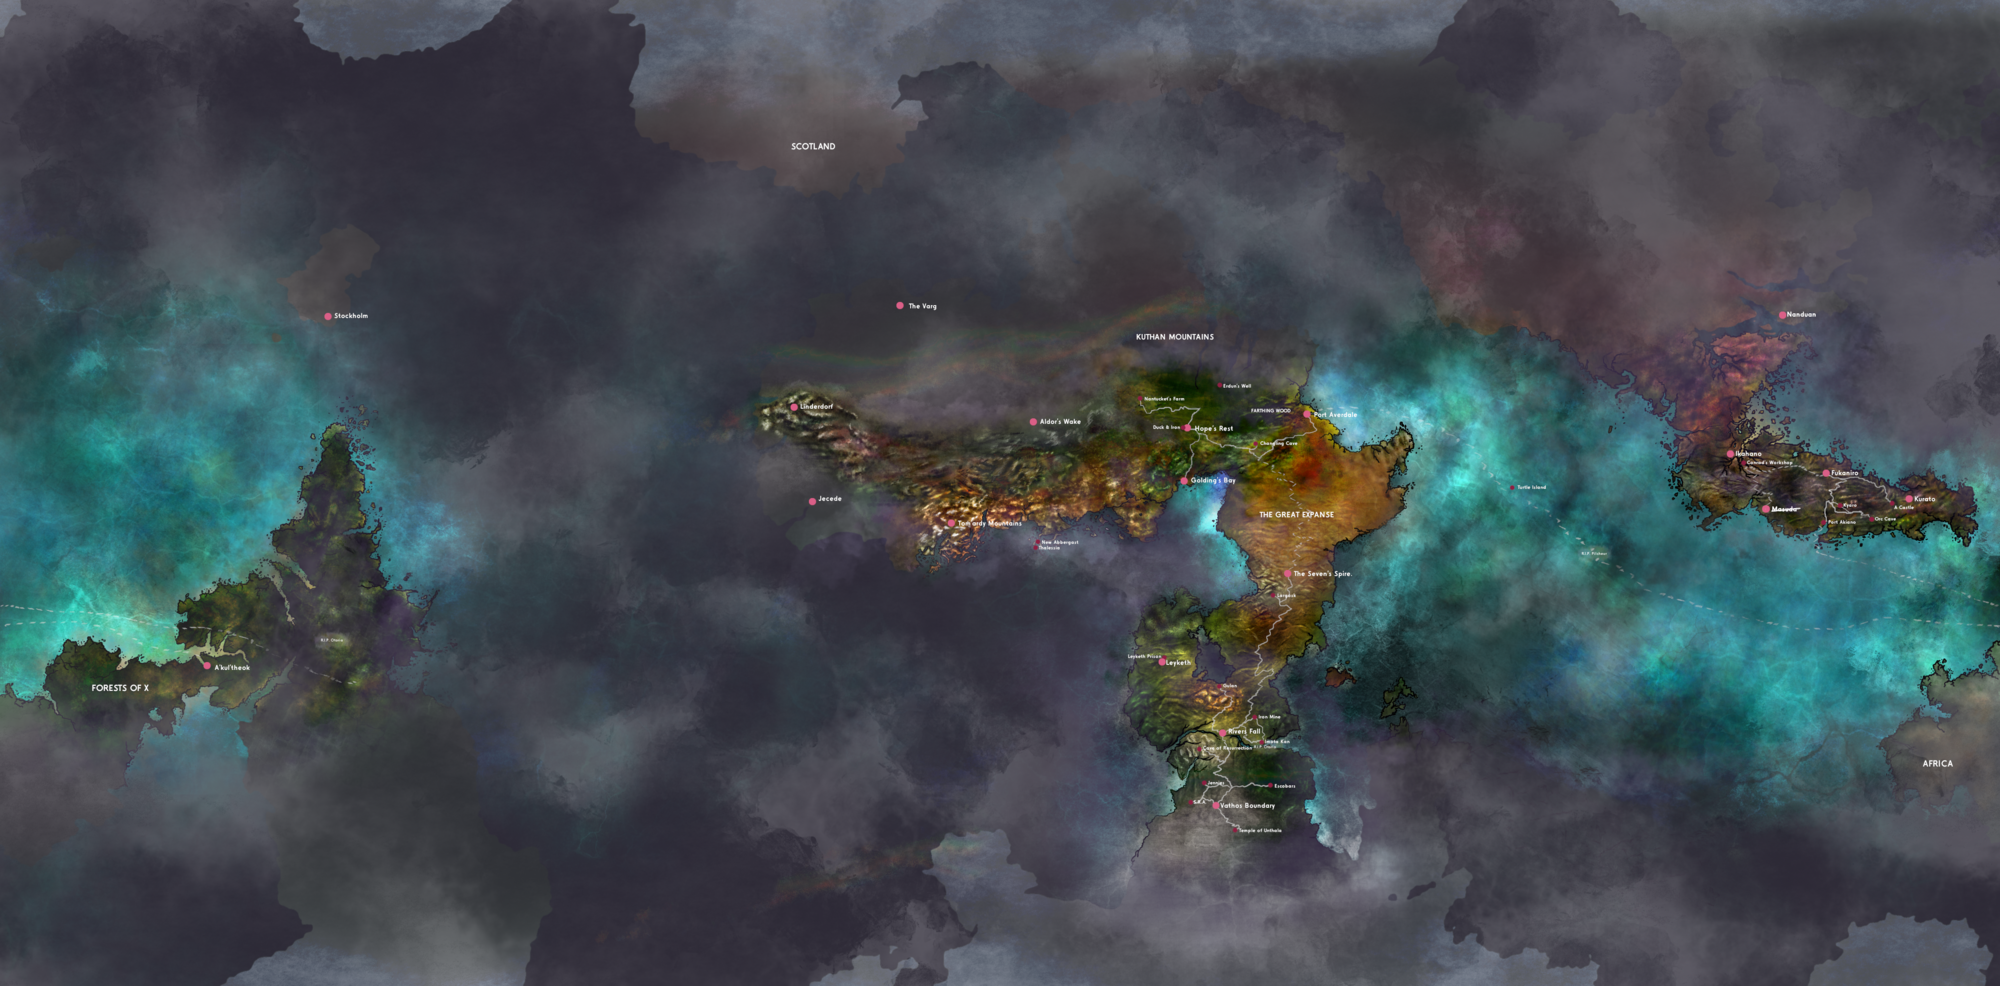
\includegraphics[width=\textwidth]{./content/img/reddit/mapEp69.png}
\begin{figure}[h]
\end{figure}
\end{center}

\clearpage
